% =====================================================================
% paper/thesis_ch5/sections/setup.tex
% §5.3 Problem description（任务 / 环境 / 传感谱系 / 特权观测 / 奖励设定 / 数据集 / 评估协议）
% =====================================================================
% rev.1（2026-06-16）：§5.3 第一批落地（§5.3.0 开篇 + §5.3.1 任务与动力学
%   + §5.3.2 可部署观测与传感谱系 + §5.3.3 特权观测）。
%   主骨架复用 paper 1 sections/setup.tex（rev.2），并据本章三线共享需求泛化：
%     - 工况：从"固定 Re150/u10 cross"泛化为亚临界 Re150/u10（λ=0.67，主工况）
%       ↔ 临界 Re250/u15（λ=1.0，边界考察）两工况；Re250 二维近似声明保留；
%     - 传感：从"s0 + 特权"补全为 s0/s1/s2 传感谱系（s0=部署主轴；s1/s2=参照上界，
%       中性陈述、不预判有用与否，守 §0.4 红线 3）；
%     - 观测维度：显式交代随奖励设定而变（历史效率导向奖励 → 40-D /
%       到达导向奖励 → 48-D），为后续各节表格维度立基。
%   术语规范（spec §0.5.10）：导航→运动规划；裸 actor/critic→策略网络（actor）/
%     价值网络（critic）；特权信息此处给具体所指 [u_eq,v_eq]（§5.1 ¶2 抽象引入，此处落地）；
%     setup 层专名解禁（涡街/REMUS/DVL/s0 等可出现）。
%   红线：s1/s2 仅作参照上界、不写"更多传感器有用/无用"；特权观测给具体值但守住
%     critic-only、部署期丢弃的可部署边界，不扩大 claim。
% rev.2（2026-06-16）：§5.3 第二批落地（§5.3.4 动作·奖励·终止 + §5.3.5 数据集
%   + §5.3.6 评估协议 + §5.3.m 实施细节与可复现性）。
%   §5.3.4 奖励设定：历史效率导向奖励作为历史离线主线背景，到达导向奖励作为
%     本章正式主奖励；迁移动机（边界提前失败套利 → 早失败惩罚抑制）已回查
%     online_sac_reward_redesign.md v6 spec 核准，不凭记忆（line 46/152/166/240/322）。
%   §5.3.5 数据集：4 类采集器（goalseek/crosscomp/世界坐标系流速补偿参照可部署
%     + 特权参照）
%     + SAC 四档 RL 采集器；主清单表 tab:ch5_datasets（精细统计下沉 §5.3.m，approved 取舍 #2）。
%   §5.3.6 评估协议：固定 manifest + Welch t / 配对自助 / rule-of-three；三条统计 cite
%     （welch1947ttest / efron1993bootstrap / jovanovic1997ruleofthree）均联网核验著录。
%   §5.3.m：obs 归一化常数 + 公共数据集规模 + 统计式 + 种子/manifest（NO APPENDIX）。
%   红线：reward map 用线/阶段语义、不硬编节号（approved 取舍 #2/#3）；privileged 采集器
%     注明特权参照不可部署；负面结果（rule-of-three 零计数上界）作 finding 同台呈现。
% rev.3（2026-06-18）：§5.3.m 公共数据集转移规模数字纠错（§5.6 起草时发现跨文档冲突，
%   经独立子 agent 核查 + 数据集 metadata.json 直证）。原值 2.4e5/4.8e5（crosscomp
%   1000/2000）、2.0e5（worldcomp 1000）系无源误推（疑把 reward spec 中 240 步 fixture
%   示例误当平均回合长度反推），与实际不符。改为实测值：crosscomp efficiency_v2
%   re150/u10cross/s0/h4 —— 1000 回合 num_transitions=152,683（≈153 步/回合，
%   offline_data metadata 直证 + dataset_diagnostics.csv + td3bc/phase0b_v2/phase0c
%   两报告四源一致）、2000 回合 304,967（报告 §3.2，本地未同步但四源确认）；worldcomp
%   efficiency_v2 同工况 1000 回合 num_transitions=104,360（≈104 步/回合，metadata 直证；
%   因 worldcomp 成功率高、路径更直，回合短于 crosscomp）。统一以“约 X×10^5”二位有效
%   数字写：1.5e5 / 3.0e5（crosscomp）、1.0e5（worldcomp）。其余 §5.3 数字（obs 归一化
%   常数、维度、种子数、回合数）非派生值、不在此次纠错范围。
% rev.4（2026-06-18）：§5.5 章级实施细节整合的配套小改（评估口径命名上提）。
%   §5.3.6 显式命名"终检评估 / 周期评估"两种评估时机，作为全章统一定义之家：
%   终检评估=训练结束后对最终检查点重评（各结果表/柱状图口径）；周期评估=训练期定期评估
%   （学习曲线口径，轻度滑动平均）。原 §5.5.m 越界承载的"三种读数全章统一"段据此瘦身、
%   只在 §5.5 就近定义在线特有的"峰值"读数。其余 §5.3 内容未动。
% 收尾统稿轮（2026-07-08）：§5.3.3 删重复括注"（critic）"×1（首现在 §5.1，
%   §0.5.10 首次括注一次规则）。机体↔船体章级统一裁定为"机体"，本节为定义之家、原文不动。
% rev.5（2026-07-24）：第 4 批 M3 落地。§5.3.5 作为**数据集定义之家**，其全场走廊参照
%   的定义原只写「读取尾流场 + 候选走廊打分 + 跟踪最优航迹」，**漏掉「以等效来流作局部
%   来流补偿」这一成分**，而 §5.8.2 的核心机制解释（闭环校正以等效来流为条件、单点瞬时
%   采样与等效来流对应关系微弱 → 条件平均把闭环校正抹平）**完全依赖它**。→ 定义补一句。
%   ⚠ 不与 §5.8.2 已有括注重复：定义之家只给**定义**（补偿成分本身），
%   §5.8.2 保留**机制**（补偿项读取的正是 eq:ch5_priv_obs 的等效来流、仅坐标系不同）。
%   零数字改动。
% rev.6（2026-07-26）：全章复审整改第 5 批（重流程；findings §10 N13 + §9 N8/N7）。§5.3.6 两处：
%   [N13·终检口径] 原定义「终检评估指训练结束后对**最终检查点**重新评估」与实际协议不符——
%     GT td3bc_phase0c_experiment_report.md §3.4 的统一选择规则是**验证集字典序选点、在独立
%     测试集上评估**（`scripts/analyze_offline_td3bc_noisy_support.py` 读 `td3bc_test_success_rate`
%     并伴随 `mean_selected_ckpt_frac` 可证），§5.6 与 §5.7 均按此执行（rebrac.tex §5.7.m 明写
%     「检查点每 8 轮保存一次，在验证集（40 回合）上按字典序规则选择」）；而 §5.5（final_eval.json）、
%     §5.8/§5.9（「直接评估训练终点检查点」）确为终点口径 → **章内同名不同义，涉两节而非一节**
%     （findings 只列 §5.6，经实核 §5.7 同病）。
%     ⚠ 改法取舍：不采「协议之家新增两个口径名 + §5.6 全节改名」（连锁广、须造新名词），
%     亦不采「§5.6 就地加一句说明」（便宜但修不好 §5.7）。采第三条路——把「终检」锚回它本来的
%     对立面（**评估时机**，终检 ↔ 周期，即 rev.4 立规时的原意），并显式声明**检查点身份是另一
%     条轴**、由各结果节在实施细节中标明（§5.4.m 早已立规）。名词由此单义、可核，一处改动同时
%     修好 §5.6 与 §5.7，零重命名、零交叉引用波及。五节所用规则均已各自标明，逐节核对无空洞。
%   [N8/N7·等价判断规则] §5.9 采分支 (b)（族内判定降为证伪框架、不作非劣判定）后，§5.3.6 的
%     条件规则在全章无兑现实例 → 补一句「本章各结果节均未作此类判断，这一附加要求因此在全章
%     不予触发」，把「有规无例」转为**显式登记的未触发条款**，承诺—兑现账本闭合。
%     ⚠⚠ **初稿写「本章各结果节均未作此类判断，该附加要求在全章不予触发」，经四维度独立
%     对抗复审判为 CRITICAL 级假陈述并已重做**（复审 B/C 独立同时命中）：§5.9.1 的数据条件
%     矩阵**确在作此类判读**（表 tab:ch5_fql_matrix 判读列两行「无差异」、正文「干净多模态
%     单元恰为无差异」、§5.9.3 亦自陈该容忍带「是为该矩阵而设」），且其 |δ|≤0.03 **确系
%     预登记** → 该附加要求是**已触发且已满足**，而非未触发；N8 的「该规则在全章已无兑现
%     实例」这一诊断前提本身即为误。定稿改为如实分档：「本章仅 §5.9.1 的数据条件矩阵作此类
%     判读，其实践容忍范围已在该节实验执行前登记；其余各结果节均只报未检测到统计显著差异，
%     该附加要求在其上不予触发。」**教训**：为使某节新框架自洽而在定义之家写下的**全称否定**，
%     极易被同章别节的表格判读列当场反证；凡在定义之家写全称句，须先对全章逐处检索该行为
%     是否存在（已写入 spec §2 §5.3 块）。同批顺手：td3bc.tex §5.6.2「与五百回合的 0.592
%     **相当**」（既有裸等价判断、命中第 3 批 H2 禁用词）改「退回五百回合的 0.592 一线」。
%   零数字改动。
% rev.7（2026-08-16）：数据完整性整改批（①③⑤ 合批，处置路径 ①-c）。§5.3 新增两个披露段，
%   均为如实登记，**零既有数字改动、零论证改动**。
%   ① §5.3.5 末新增一段，写明离线数据集与固定评估集的种子区间关系：采集自种子 0 起为每个
%     回合连续编号、主评估集固定取 1250–1349，故 ≤1000 回合的数据集与评估集不相交；而 2000
%     回合规模（历史效率导向确定性集 + §5.6.2 支持集诊断所用的同规模含噪变体）种子区间
%     0–1999 完整覆盖评估区间 → 该规模上训练与终检的任务实例逐条相同。
%     证据：两个数据集 metadata.json 的 seed/num_episodes + reset RNG 重放的实例级比对
%     （flow_time/start_xy/goal_xy/initial_heading 四项在 1e-6 容差下 100/100 一致），
%     两集均已实核（含噪 2000 集此前从未进过污染面枚举，2026-08-16 Drive 侧补核）。
%   ② §5.3.6 新增一段，写明选点验证集是终检评估集的**固定前 40 条子集**（任务实例嵌套而非
%     独立采样），且筛查协议（val/test 各 40 回合）下两者为同一批实例；并声明已作「仅在
%     未参与选点的后 60 条上重算」的事后复核。措辞与 §5.8 既有先例同构（boundary.tex:188/258
%     「30 回合集为 100 回合主评估集的固定前 30 条子集，两者的任务实例嵌套而非彼此独立」），
%     属同类披露的口径统一，而非新立说法。
%   量化读数一律不写入本节，集中登记于 §5.7.m——定义之家不承载结果数字（承 rev.5 的分工）。
% rev.8（2026-08-16）：整改批的独立对抗复审整改（复审判 MED-2）。本节一处，零数字改动。
%   §5.6.3 的复核声明由**全称**收窄为**枚举口径**：原「把**每个**终检读数……重算**各处**组间
%   比较……不改变**本章任何**结论的方向」→ 明写复核面为按验证集指标选点的各单元（§5.6/§5.7
%   两节），并声明 §5.5/§5.8/§5.9 均直接评估训练终点检查点、不作验证集选点，不在该嵌套影响
%   之列；末句限定为「在 §5.7.m 所枚举的范围内」。
%   ⚠ 触发原因：源头 §5.7.m 用的是闭合枚举（「本章相关比较……：」+ 四项 + 一例外），本节与
%     §5.10.4 却把它universal 化。且 §5.8 亚临界一侧的 30 回合评估集整体落在前 40 条之内，
%     结构上无留出回合可拆——「每个终检读数」经不起追问（已就地写明）。
%   本机另有一处无法覆盖：world 特权 ReBRAC-Q 单元 seeds 45/46 的 test json 未同步本机
%     （rev.3 头注已记），该单元不在复核枚举内；改后措辞不再声称覆盖它。
% =====================================================================

\section{问题设定与评估协议}\label{sec:ch5_setup}

本章三条研究线——在线可学性、离线主线与算法对比——共享同一套任务、环境与部署接口。本节固定这一设定，并明确贯穿全章的四条对照轴：奖励目标、流动工况、传感配置与数据采集器。这一设定同时给出中心命题两侧的具体所指：策略在部署时实际掌握的信息，仅是 AUV 单点处的局部流速估计；可供离线学习复用的数据，是既有控制器采集的轨迹；而为系统增添能力的若干途径中，有两条可在本节的环境与接口层面精确定义，即增设空间探针与向价值网络注入特权观测；第三条途径，采用更具表达力的策略先验，属算法层面，留待方法节界定。全章结果表格中的奖励、工况与传感维度均以本节为基准。

\subsection{任务与动力学}\label{subsec:ch5_task}

本章考虑一类水下自主航行器在卡门涡街（Kármán vortex street）尾流场中执行点到点运动规划的任务。航行器为 REMUS-100 类圆柱形载体（长 $L=1.6$ m，直径 $d=0.19$ m，排水质量 $m\approx 32$ kg），其动力学采用 Fossen 框架下完整的六自由度非线性方程组~\citep{fossen2011handbook}，含附加质量、科氏力、横流阻力、桨叶推力与舵面升力，以四阶 Runge--Kutta 积分器在物理步长 $\Delta t_{\mathrm{sim}}=0.1$ s 上推进；每个决策步含 5 个物理子步，对应控制周期 $\Delta t_{\mathrm{ctrl}}=0.5$ s。深度由级联 PID 内环维持，使六自由度动力学在水平面退化为有效的三自由度平面运动 $[u,v,r,x_N,y_E,\psi]$。

尾流场由二维双弛豫时间格子玻尔兹曼方法离线生成，圆柱直径 $D=12$ m，输出空间分辨率 $\Delta x=0.6$ m，记录时长约 $360$ s（覆盖约九至十个涡旋脱落周期），每回合起始相位在记录区间内均匀随机采样以避免相位过拟合。本章在两个流动工况上考察策略。亚临界工况取来流 $U_\infty=1.0$ m/s、雷诺数 $\mathrm{Re}=150$，处于严格的二维层流卡门涡街区间，是全章的主工况；临界工况取 $U_\infty=1.5$ m/s、$\mathrm{Re}=250$，涡旋更强、脱落更快，专用于刻画策略的失效边界。需说明的是，真实绕流在 $\mathrm{Re}\approx 190$ 处发生三维失稳，$\mathrm{Re}=250$ 仍采用二维模型是一处明确的建模简化：它略微高估涡旋强度与斯特劳哈尔数，但不改变卡门涡街的定性时空结构。

任务几何以垂直来流方向（$\pm 20^\circ$ 内随机）的横流穿越为主，目标对水速度上限 $V_{\max}=1.5$ m/s。两个工况下的速度比 $\lambda=U_\infty/V_{\max}$ 分别为 $0.67$ 与 $1.0$。当 $\lambda=1.0$ 时，航行器在自由来流中可用于形成稳定对地位移的速度余量显著收缩，单纯按来流作直线补偿难以保证横流穿越任务中的净位移，因而需要利用尾流的非均匀结构——低速走廊、瞬态反向流与交变横向分量——获得可行运动。每回合起终点距离在 $[40,90]$ m 内均匀采样，质心进入目标 $4$ m 半径内判成功，越出流场边界、动力学违规或超时（$240$ s）判失败。

\subsection{可部署观测与传感谱系}\label{subsec:ch5_obs_deployable}

策略在每个决策步接收的可部署观测 $\mathbf{o}_t$ 由本体状态、目标信息与局部流速三部分拼接而成。本体五维为体轴线速度与偏航率 $(u,v,r)$ 以及以 $(\cos\psi,\sin\psi)$ 编码的艏向（三角编码避免 $\pm\pi$ 跳变）；目标三维为目标在体坐标系下的相对位置 $(\Delta x_b,\Delta y_b)$ 与距离 $d$，各量按固定尺度归一化，体坐标系表示使观测对全局朝向具有不变性。流速部分由探针布局决定：每个探针给出其所在位置体坐标系下的单点流速 $(u_c,v_c)$。

本章涉及三种探针布局，均对应 REMUS-100 平台上物理可实现的传感配置（表~\ref{tab:ch5_sensor_family}，探针几何见图~\ref{fig:ch5_sensor_family}）。$s_0$ 仅在机体质心 $(0,0)$ 设单一探针，对应平台标配的多普勒测速仪（DVL，1200 kHz）水追踪模式所能给出的最弱流场感知——它只测得当前位置的瞬时流速，是单点流速测量的下界。这一布局是本章策略网络（actor）在三条研究线中共享的部署主轴，也正是中心命题中策略可资利用的已有信息的物理载体。$s_1$ 在 $s_0$ 之外增设一处前向探针 $(4.5,0)$，对应一台 2 MHz 短程 ADCP，提供约三个控制步的轴向预警；$s_2$ 进一步增设近端与两侧探针 $(5,0)$、$(8,\pm 4)$，对应 1 MHz 长程 ADCP，兼具约七步的轴向预警与侧向流速梯度感知。$s_1$ 与 $s_2$ 在本章中仅作物理可对应的参照上界，用以界定 $s_0$ 与更丰富空间感知之间的差距；本节不预设额外空间感知对可部署性能的必要性。

观测在送入策略前外接 $k=4$ 步历史堆叠，以时间维度补偿单点感知缺失的空间信息。本章奖励设定在观测构成上仅有一处差异：到达导向奖励额外附带两个回合级上下文通道（已耗时间占比与归一化初始距离），历史效率导向奖励则无；这一差异来自到达导向奖励对时间语义与初始距离尺度的显式编码。因此 $s_0$ 单步观测在历史效率导向奖励下为 $10$ 维、在到达导向奖励下为 $12$ 维，经 $k=4$ 历史堆叠后分别为 $40$ 维与 $48$ 维；各结果表中的观测维度均以此为准。

\begin{table}[t]
\centering
\caption{本章的三种传感配置。三者均对应 REMUS-100 平台上物理可实现的传感器；$s_0$ 是全章策略网络共享的可部署主轴，$s_1$ 与 $s_2$ 仅作参照上界。单步观测维度为 $8$（本体 $5$ + 目标 $3$）$+\,2n_p$（$n_p$ 为探针数），到达导向奖励另加 $2$ 个回合级上下文通道（见正文）。}
\label{tab:ch5_sensor_family}
\begin{tabular}{l l l >{\raggedright\arraybackslash}p{0.30\linewidth}}
\toprule
\textbf{布局} & \textbf{探针位置（体轴，m）} & \textbf{物理对应传感器} & \textbf{角色 / 感知类型} \\
\midrule
$s_0$ & $(0,0)$ & DVL 1200 kHz 水追踪 & 可部署主轴；单点瞬时流速 \\
$s_1$ & $(0,0),\,(4.5,0)$ & $+$ 2 MHz 短程 ADCP & 参照上界；短程预警（$\sim 3$ 步）\\
$s_2$ & $(0,0),\,(5,0),\,(8,\pm 4)$ & $+$ 1 MHz 长程 ADCP & 参照上界；长程预警（$\sim 7$ 步）与侧向梯度 \\
\bottomrule
\end{tabular}
\end{table}

\begin{figure}[t]
    \centering
    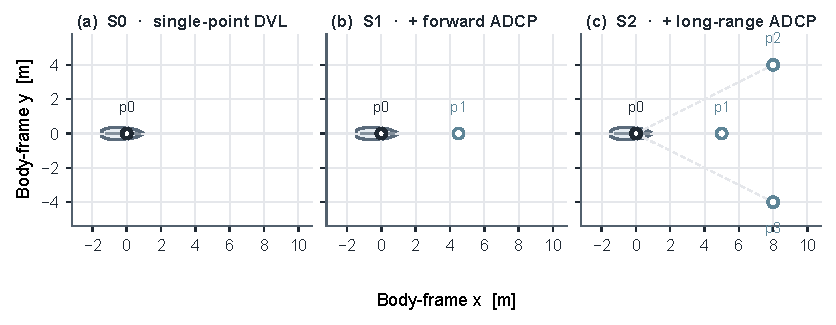
\includegraphics[width=138mm]{figures/fig_ch5_sensor_family.pdf}
    \caption{本章三种传感配置的体坐标系探针几何。(a) $s_0$ 仅在机体质心设单一 DVL 水追踪探针，是可部署主轴；(b) $s_1$ 在 $s_0$ 之外增设一处前向探针（机体前方 $4.5$ m），对应短程前视 ADCP，提供约三个控制步的轴向预警；(c) $s_2$ 进一步增设近端前向（$5$ m）与两侧（纵向 $8$ m、横向 $\pm 4$ m）探针，对应长程前视 ADCP，兼具约七步的轴向预警与侧向流速梯度。实心圆为质心单点探针，空心圆为增设的前向／侧向探针；$s_1$ 与 $s_2$ 仅作物理可对应的参照上界。}
    \label{fig:ch5_sensor_family}
\end{figure}

\subsection{特权观测（仅价值网络）}\label{subsec:ch5_obs_privileged}

为支持非对称 Actor-Critic~\citep{pinto2017asymmetric} 协议下的对照，环境另给出一路特权观测 $\mathbf{o}_t^{\mathrm{priv}}\in\mathbb{R}^2$。它是 \S\ref{sec:ch5_intro} 中抽象引入的特权信息在本任务中的具体所指，即体坐标系下的沿机体采样等效来流 $(u_{\mathrm{eq}},v_{\mathrm{eq}})$。这里的等效来流由沿 AUV 机体纵轴若干代表点采样平均得到，而非全场流场输入；其数值由沿机体纵轴 $N=5$ 个等距采样点的世界系流速等权平均、再投影至体坐标系给出：
\begin{equation}
\mathbf{o}_t^{\mathrm{priv}} = (u_{\mathrm{eq}},\,v_{\mathrm{eq}})
= \frac{1}{N}\sum_{i=1}^{N} R_{wb}(\psi)\,\mathbf{u}_{\mathrm{world}}\!\left(\mathbf{p}^{(0)} + \xi_i\, L\,\hat{\mathbf{e}}_{\mathrm{body}}\right),
\qquad \xi_i \in \{-0.4,\,-0.2,\,0,\,0.2,\,0.4\}.
\label{eq:ch5_priv_obs}
\end{equation}
其中 $R_{wb}(\psi)$ 为世界系到体坐标系的旋转矩阵。该量等价于求解六自由度方程时实际作用于载体的有效来流，因而是物理含义明确的动力学有效输入，而非与动力学无关的任意隐藏变量；它在训练期可得、部署期不可得，恰是特权信息的定义性特征。与之相对，可部署观测中的单点流速只是探针所在位置的瞬时采样，并不等于驱动六自由度动力学的等效来流；二者之间的这一系统性信息落差，正是后续各方法比较所围绕的核心信息边界。

据此区分两种训练协议。可部署协议下，策略网络与价值网络都只读 $\mathbf{o}_t$，与本章定义的 REMUS-100 可部署传感接口一致；特权协议下，价值网络额外读取 $\mathbf{o}_t^{\mathrm{priv}}$，而策略网络始终只读 $\mathbf{o}_t$。评估与部署阶段价值网络已被弃用，$\mathbf{o}_t^{\mathrm{priv}}$ 不出现在执行回路中，故两种协议训练所得策略在部署时的传感依赖完全一致。图~\ref{fig:ch5_sensor_schematic} 示意了任务几何与两种协议下两个网络的传感边界。这一对照正是本章检验特权信息是否必需的实验杠杆：若可部署协议达到与特权协议相近的性能，则训练期额外提供的等效流速信息对部署性能并非必需。

\begin{figure}[t]
    \centering
    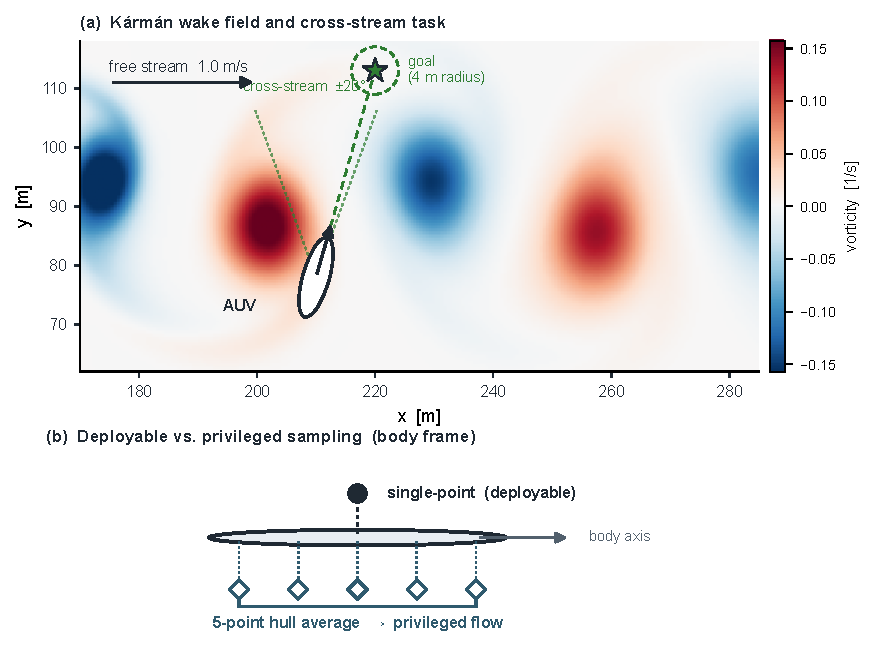
\includegraphics[width=138mm]{figures/fig_ch5_sensor_schematic.pdf}
    \caption{任务与传感协议示意。(a) 亚临界工况（$U_\infty=1.0$ m/s、$\mathrm{Re}=150$、湍流强度 $5\%$）某一帧的涡量背景，叠加 REMUS-100 体示意（白色椭圆，箭头为艏向）、横流穿越目标（绿色五角星）及其 $4$ m 成功半径，与垂直来流 $\pm 20^\circ$ 的横流穿越方向锥；每回合起终点距离在 $40$--$90$ m 内随机采样。(b) 体坐标系下两种传感抽样协议（按比例）：实心圆 $s_0$ 是部署可得的单点 DVL 水追踪，策略网络在两种协议下都只读此通道；空心菱形为沿体轴 $\xi_i\in\{-0.4,-0.2,0,+0.2,+0.4\}\cdot L$ 的五个等距采样点，等权平均后给出沿机体采样等效来流 $\mathbf{o}^{\mathrm{priv}}=[u_{\mathrm{eq}},v_{\mathrm{eq}}]$，仅在特权协议训练阶段被价值网络读取，部署阶段不可用（\eqref{eq:ch5_priv_obs}）。}
    \label{fig:ch5_sensor_schematic}
\end{figure}

\subsection{动作、奖励与终止}\label{subsec:ch5_reward}

航行器的动作为二维连续向量 $\mathbf{a}_t=(a_\psi,a_n)\in[-1,1]^2$。在绝对航向模式下，$a_\psi$ 映射为期望偏航角参考 $\psi_{\mathrm{ref}}=a_\psi\cdot\pi$，由内层 PD 控制器跟踪；$a_n$ 映射为归一化的螺旋桨转速指令。这两个分量分别支配航向选择与推进强度，构成策略借流机动的全部操纵自由度。

本章正式采用到达导向奖励作为任务成功率分析的主奖励设定。为说明其设计必要性，先回顾历史效率导向奖励，即离线主线早期所采用的奖励设定。该奖励以时间惩罚和目标距离进度整形为主体，并叠加轻量软安全代价与终止奖励；它适合在早期行为约束离线方法之间保持同口径比较，但在较难任务中可能产生目标错配：当策略难以到达目标时，持续累积的时间惩罚可能使提前越界获得比长时间接近目标更高的回报。

历史效率导向奖励由四项叠加构成，即每步时间惩罚、基于目标距离差的进度整形、轻量软安全惩罚以及终止奖励：
\begin{equation}
r_t \;=\; \underbrace{-\,c\,\Delta t_{\mathrm{ctrl}}}_{\text{时间惩罚}}
       \;+\; \underbrace{k_p\,(d_{t-1}-d_t)}_{\text{进度整形}}
       \;-\; \underbrace{k_s\,c_t^{\mathrm{safety}}}_{\text{软安全惩罚}}
       \;+\; r_{\mathrm{term}},
\qquad c = 2.0\ \mathrm{s}^{-1},\quad k_p = 1.0,\quad k_s=0.25,
\label{eq:ch5_reward_eff}
\end{equation}
终止奖励 $r_{\mathrm{term}}$ 为到达目标的 $+100$ 或失败的 $-20$，越界、动力学违规与超时均判失败；$c_t^{\mathrm{safety}}$ 为边界、姿态、速度与角速度风险的统一软代价。尽管该软安全项已对贴近边界的行为给出惩罚，其权重相对每步时间惩罚与终止项较弱。在较难任务中，这一奖励结构可能诱发一种退化模式：当目标在当前策略下难以到达时，持续累积的每步时间惩罚使提前越界成为回报更优的选择，失败惩罚 $-20$ 与轻量安全项不足以抵消长时间漂行累积的时间代价，策略遂可能贴边滑行并尽早触发越界终止，使回合回报与任务成功率之间出现错配。这一沿边界提前失败的回报偏置暴露出历史效率导向奖励与任务主指标的错配，促成了向到达导向奖励的迁移。

基于这一失配，本章正式的可学习性分析、泛化边界考察与算法比较统一采用到达导向奖励；历史效率导向奖励则保留于离线主线与既有结果的同口径对照，以及在线情形下早期的传感配置可行性筛查（其结论限于配置间的相对可学习性）。到达导向奖励不再把“更快结束”作为隐含优化方向，而是显式区分到达、超时与硬失败，并通过早失败惩罚抑制快速越界。每步奖励给出归一化的进度整形、微弱的时间代价与软安全惩罚：
\begin{equation}
r_t^{\mathrm{step}} \;=\; w_p\,\frac{d_{t-1}-d_t}{d_0}
\;-\; w_\tau\,\frac{\Delta t_{\mathrm{ctrl}}}{T_{\max}}
\;-\; w_s\,c_t^{\mathrm{safety}},
\label{eq:ch5_reward_arrival_step}
\end{equation}
回合终止时按语义附加终止项
\begin{equation}
r^{\mathrm{term}} \;=\;
\begin{cases}
+\,R_{\mathrm{succ}}, & \text{到达目标},\\[2pt]
-\,R_{\mathrm{to}} \;-\; R_d\,\rho, & \text{超时},\\[2pt]
-\,R_{\mathrm{fail}} \;-\; R_{\mathrm{early}}\,(1-\eta) \;-\; R_d\,\rho, & \text{硬失败},
\end{cases}
\label{eq:ch5_reward_arrival_term}
\end{equation}
其中 $d_0=\max(d_{\mathrm{init}},10\,\mathrm{m})$ 为带下界保护的初始目标距离，$\eta=\mathrm{clip}(t/T_{\max},0,1)$ 为已耗时间占比，$\rho=\mathrm{clip}(d_t/d_0,0,2)$ 为终止距离比；本章任务的起终点距离为 $40$--$90$ m，故该下界保护在正式评估分布内不激活。权重取 $w_p=50$、$w_\tau=5$、$w_s=2$，终止系数 $R_{\mathrm{succ}}=R_{\mathrm{fail}}=R_{\mathrm{early}}=100$、$R_{\mathrm{to}}=R_d=50$。

两处设计共同抑制了上述提前失败偏置。硬失败的早失败惩罚 $R_{\mathrm{early}}(1-\eta)$ 随已耗时间递减，使越早越界惩罚越重；该奖励设计满足的核心约束是，成功优于超时、超时优于硬失败，尤其快速越界不再优于接近目标的超时回合。同时，归一化的进度与时间项把每步信号压到低于终止项的量级，使任务语义主要由到达、超时与硬失败三类终止项表达，而不再由累积步惩罚主导。代价是奖励不再是纯势函数整形：到达、超时与硬失败的非势函数终止项直接编码任务语义，这一取舍意在换取与主指标对齐的可学习信号。两个回合级量（已耗时间占比 $\eta$ 与按固定距离尺度归一化的初始目标距离）须进入观测，否则同一转移会因隐藏的已耗时间或初始距离获得不同回报，破坏价值函数的马尔可夫性；这正是到达导向奖励观测较历史效率导向奖励多两维的原因（\S\ref{subsec:ch5_obs_deployable}）。历史效率导向奖励在上述保留用途中的回报数值不与到达导向奖励下的回报作直接比较；跨设定讨论只限于任务成功率、部署约束、信息利用和失效边界等机制性结论。

\subsection{数据集}\label{subsec:ch5_datasets}

离线数据由若干行为策略在上述环境中采集。目标直指参照与横流补偿参照是严格的 $s_0$ 非学习控制器，前者直接朝目标航行并固定油门，后者依单点流速的体坐标系横向分量做反向偏航补偿；二者与待训练策略共享最弱传感协议。世界坐标系流速补偿参照作为理想化的可部署流速补偿基线，使用世界坐标系下的当前等效流速估计修正期望对地航迹；它不读取未来流场或全场候选走廊，但其信息口径强于仅由策略观测向量直接解码的严格单点观测控制器。全场走廊参照读取仿真器尾流场，为若干候选走廊打分并跟踪最优航迹，并以等效来流估计对局部来流作补偿；它本身不可部署，仅用于生成高质量的参照数据。这里的全场走廊参照是行为数据采集器，不等同于 \S\ref{subsec:ch5_obs_privileged} 中仅供价值网络读取的特权观测协议。

除上述规则型策略外，本章还引入由在线 SAC 策略检查点构成的采集器族。沿用离线强化学习基准构造数据的通行做法，从一条 SAC 训练轨迹的不同阶段截取检查点，得到质量递增的四档采集器（随机、中等、中等偏专家、专家），其行为策略与 $s_0$ 部署传感保持一致。这一数据源服务于算法对比线索，用以考察算法表现如何随数据质量变化，并提供规则型采集器覆盖不到的中等质量工况。

表~\ref{tab:ch5_datasets} 汇总本章主要离线数据集及其在四条对照轴——采集器、奖励设定、工况、传感——上的坐标，并标明各自用途。所有数据集统一采用 $s_0$ 传感、$k=4$ 历史与横流穿越几何，每集 $1000$ 回合（历史效率导向数据集另含一个 $2000$ 回合预算）；差异集中在采集器（数据质量）、奖励目标与流动工况三轴。公共数据集的转移规模列于 \S\ref{subsec:ch5_impl}，其余逐档统计随相应实验条件报告。

离线数据集与固定评估集的任务实例都由随机种子唯一确定，且经同一套采样机制生成，二者的种子区间关系须在此写明。数据采集自种子 $0$ 起为每个回合连续编号，主评估集的 $100$ 个任务实例则固定取种子 $1250$ 至 $1349$（\S\ref{subsec:ch5_eval}）。一千回合及以下的数据集其种子区间止于 $999$，与评估集不相交；而两千回合规模的数据集——表~\ref{tab:ch5_datasets} 所列的历史效率导向 $2000$ 回合集，以及 \S\ref{subsec:ch5_td3bc_support} 支持集诊断所用的同规模含噪变体——其种子区间 $0$ 至 $1999$ 完整覆盖评估集的种子区间，该规模上的训练任务实例因而与终检评估的任务实例逐条相同。这一重合限于两千回合一档，其对相关结论的影响在 \S\ref{subsec:ch5_td3bc_support} 与 \S\ref{subsec:ch5_rebrac_scale} 各自就地界定，量化读数集中登记于 \S\ref{subsec:ch5_rebrac_impl}。

\begin{table}[t]
\centering
\caption{本章主要离线数据集及其在采集器、奖励设定、流动工况与规模四轴上的坐标，并兼作共享设定的复现索引。所有数据集共享 $s_0$ 传感与 $k=4$ 历史堆叠，观测维度由奖励设定决定（历史效率导向奖励为 $40$ 维、到达导向奖励为 $48$ 维）；离线主线固定 $5$ 个随机种子，其余各线在各自协议内使用固定种子组，评估回合数与固定评估集见 \S\ref{subsec:ch5_eval}。FQL 的多模态与含噪变体、SAC 各档统计作为相应实验条件的一部分另行报告。}
\label{tab:ch5_datasets}
\begin{tabular}{>{\raggedright\arraybackslash}p{0.17\linewidth} l l c >{\raggedright\arraybackslash}p{0.20\linewidth}}
\toprule
\textbf{采集器} & \textbf{奖励设定} & \textbf{工况} & \textbf{回合数} & \textbf{用途} \\
\midrule
横流补偿参照 & 历史效率导向奖励 & 亚临界（$\mathrm{Re}{=}150$） & 1000 / 2000 & 历史效率导向离线主线数据 \\
世界坐标系流速补偿参照 & 历史效率导向奖励 & 亚临界（$\mathrm{Re}{=}150$） & 1000 & 可部署–特权协议对照 \\
横流补偿参照 & 到达导向奖励 & 亚临界（$\mathrm{Re}{=}150$） & 1000 & 亚临界到达任务数据 \\
全场走廊参照 & 到达导向奖励 & 临界（$\mathrm{Re}{=}250$） & 1000 & 临界到达任务数据 \\
全场走廊参照 & 到达导向奖励 & 亚临界（$\mathrm{Re}{=}150$） & 1000 & 高质量到达任务数据 \\
SAC 检查点（四档） & 到达导向奖励 & 亚临界（$\mathrm{Re}{=}150$） & 1000 & 数据质量对照轴 \\
\bottomrule
\end{tabular}
\end{table}

\subsection{评估协议}\label{subsec:ch5_eval}

所有方法在固定评估集（manifest）上以确定性策略评估。评估集是一组预先采样、各方法共用的起终点与流场相位配置，使不同算法、不同种子的成功率严格可比，其任务分布与对应数据采集时一致。全章区分两种评估时机：\emph{终检评估}指训练结束后在评估集上对该次训练选定的检查点重新评估，是各结果表与柱状图所报成功率的统一口径；所选定的检查点或为训练终点检查点，或为训练期保存的检查点中按验证集指标的字典序选出者（\S\ref{subsec:ch5_method_impl}），各结果节在其实施细节中标明所用规则。\emph{周期评估}指训练期间每隔固定步数对当前检查点的评估，用于绘制学习曲线，绘图时经轻度滑动平均以抑制评估噪声。本章正式的到达导向主评估集在主工况每种子 $100$ 回合，较难工况与训练期周期评估每种子 $30$ 回合；主指标为任务成功率，即质心进入目标半径内的回合占比。在线情形下早期采用历史效率导向奖励的传感配置筛查另用其自身的评估集，其回合数在 \S\ref{sec:ch5_online} 就近说明。

选点所用验证集与终检评估集之间存在固定的包含关系，须在此一并写明。两者由同一评估集配置生成：验证集取其固定前 $40$ 条任务实例，终检评估集取前 $100$ 条，任务实例嵌套而非彼此独立；在验证与测试各取 $40$ 回合的筛查协议下（\S\ref{subsec:ch5_rebrac_impl}），两者更是同一批任务实例。因此终检所报的 $100$ 个回合中，有 $40$ 个曾参与检查点选择。为界定这一嵌套对相关比较的影响，本章对受其影响的已报结果作了一项事后复核：把终检读数按种子拆成参与过选点的前 $40$ 条与选点规则未见的后 $60$ 条（下称留出回合），仅在留出回合上重算组间比较。复核面即按验证集指标选点的各单元，集中于 \S\ref{sec:ch5_td3bc} 与 \S\ref{sec:ch5_rebrac} 两节；\S\ref{sec:ch5_online}、\S\ref{sec:ch5_boundary} 与 \S\ref{sec:ch5_algo_compare} 均直接评估训练终点检查点、不作验证集选点，不在该嵌套的影响之列（其中 \S\ref{sec:ch5_boundary} 亚临界一侧的 $30$ 回合评估集整体落在上述前 $40$ 条之内，本也无留出回合可拆）。复核的逐项枚举与量化读数集中登记于 \S\ref{subsec:ch5_rebrac_impl}；在该枚举范围内，除一处比例读数外，它不改变已报结论的方向。

成对协议的比较（如可部署协议与特权协议）以随机种子为主要推断单位：每个种子先在固定评估集上得到成功率，再比较种子级均值。两组独立的种子级成功率均值之差以 Welch 不等方差 $t$ 检验判别~\citep{welch1947ttest}，自由度按 Welch--Satterthwaite 公式计算。回合级配对自助法仅作为固定评估集下对配对任务实例的敏感性复核~\citep{efron1993bootstrap}，即在保持方法配对关系的前提下对评估任务实例重采样，报告均值差的百分位置信区间，用于检查结论是否依赖少数起终点或流场相位；它不替代种子级推断，也不把回合视为独立推断样本。当 $t$ 检验不拒绝等均值且自助置信区间跨越零时，本章表述为未检测到统计显著差异；若进一步作出性能相近或等价判断，则同时要求种子级效应量落在相应结果节预先给出的实践容忍范围内。本章仅 \S\ref{subsec:ch5_algo_matrix} 的数据条件矩阵作此类判读，其实践容忍范围已在该节实验执行前登记；其余各结果节均只报未检测到统计显著差异，该附加要求在其上不予触发。

对成功率为零的负面结果，单凭点估计不足以界定其上界。本章按 rule-of-three 给出此类零计数的 $95\%$ 置信上界约 $3/n$~\citep{jovanovic1997ruleofthree}，使“完全失败”这一结论本身带有量化的统计强度，与正面结果同台呈现而非降格为附带说明。随机种子取固定数量的一组，全章各线在其协议内保持一致；正文报告种子数量和每种子评估回合数，具体随机种子编号保留在复现实验配置与结果记录中。

\subsection{实施细节与可复现性}\label{subsec:ch5_impl}

观测各通道的归一化常数为：速度尺度 $2.0$ m/s（本体与流速通道共用）、偏航率尺度 $1.0$ rad/s、距离尺度 $200$ m。到达导向奖励的两个回合级上下文通道分别为已耗时间占比 $\eta\in[0,1]$ 与按 $200$ m 归一化的初始目标距离。特权观测 $\mathbf{o}^{\mathrm{priv}}=[u_{\mathrm{eq}},v_{\mathrm{eq}}]$ 维度为 $2$、不随历史堆叠，离线数据以 $\mathbf{o}^{\mathrm{priv}}$ 与其后继 $\mathbf{o}'^{\mathrm{priv}}$ 两列随转移一并记录，以支持接收特权观测的价值网络协议。

公共数据集的规模如下：横流补偿参照的 $1000$ / $2000$ 回合集分别约含 $1.5\times10^5$ / $3.0\times10^5$ 条转移，世界坐标系流速补偿参照的 $1000$ 回合集约 $1.0\times10^5$ 条。到达导向奖励下的基线采集器与 SAC 检查点采集器同样以 $1000$ 回合为基本规模；SAC 四档采集器的逐档转移条数、行为质量与失败模式分布在算法对比分析中给出。

Welch--Satterthwaite 自由度由两组样本方差与样本量按标准公式计算；配对自助法取 $B=10^4$ 次回合级重采样给出百分位置信区间。固定评估集按工况组织：主工况评估集为亚临界横流穿越配置（目标对水速度 $1.5$ m/s，每种子 $100$ 回合），较难工况评估集为临界工况配置（$\mathrm{Re}=250$、$U_\infty=1.5$ m/s，每种子 $30$ 回合）。离线主线固定 $5$ 个随机种子，泛化边界与算法对比在各自协议内使用固定种子组；具体随机种子编号不作为正文论证对象，保留于复现实验配置。
